\documentclass[letterpaper]{article}

\usepackage{graphicx}  %Required
\usepackage{multirow}
\usepackage{amsmath,amsfonts,amssymb}
\usepackage[left=2cm, right=2cm, top=2cm]{geometry}

\title{Supplemental Material:\\Disentangled Representation Learning for\\Non-Parallel Text Style Transfer}


\date{}
\author{}
\begin{document}
\maketitle
\graphicspath{{images/}}

% used for table headers
\newcommand{\tabh}[1]{\multicolumn{1}{c|}{\textbf{#1}}}
% used for the top left cell in a table
\newcommand{\tabc}[2]{\multicolumn{1}{|c||}{\multirow{#1}{*}{\textbf{#2}}}}

\newcommand{\loss}[1]{J_{\text{#1}}}

\section{Bag-of-Words (BoW) Vocabulary Ablation Tests}

The tests in Table \ref{tab:bow-vocab-ablation} demonstrate the effect of the choice of vocabulary used for the auxiliary content losses.

\begin{table}[ht]
	\centering
	\begin{tabular}{| l || c | c | c | c |}
		\hline
		\tabc{2}{BoW Vocabulary}                         & \tabh{Transfer} & \tabh{Cosine}     & \tabh{Word}    & \tabh{Language} \\
		                                                 & \tabh{Strength} & \tabh{Similarity} & \tabh{Overlap} & \tabh{Fluency}  \\
		\hline
		\hline
		Full Corpus Vocabulary                           & 0.822           & 0.896             & 0.344          & -10.13          \\
		\hline
		Vocabulary without sentiment words               & 0.872           & 0.901             & 0.359          & -10.33          \\
		\hline
		Vocabulary without stopwords                     & 0.836           & 0.894             & 0.429          & -10.06          \\
		\hline
		Vocabulary without stopwords and sentiment words & \textbf{0.934}  & \textbf{0.904}    & \textbf{0.473} & \textbf{-9.84}  \\
		\hline
	\end{tabular}
	\caption{Ablation tests on the BoW vocabulary.}
	\label{tab:bow-vocab-ablation}
\end{table}

It is evident that using a BoW vocabulary that excludes sentiment words and stopwords performs better on every single quantitative metric.


\section{t-SNE plots of Ablation Tests}

Figure \ref{fig:only-rec} shows the t-SNE plots of the style and content embeddings, without any auxiliary losses.
Figures \ref{fig:rec-and-muls}, \ref{fig:rec-and-advs}, \ref{fig:rec-and-mulc} and \ref{fig:rec-and-advc} show the effect of adding each of the auxiliary losses independently.

\begin{figure}[ht]
	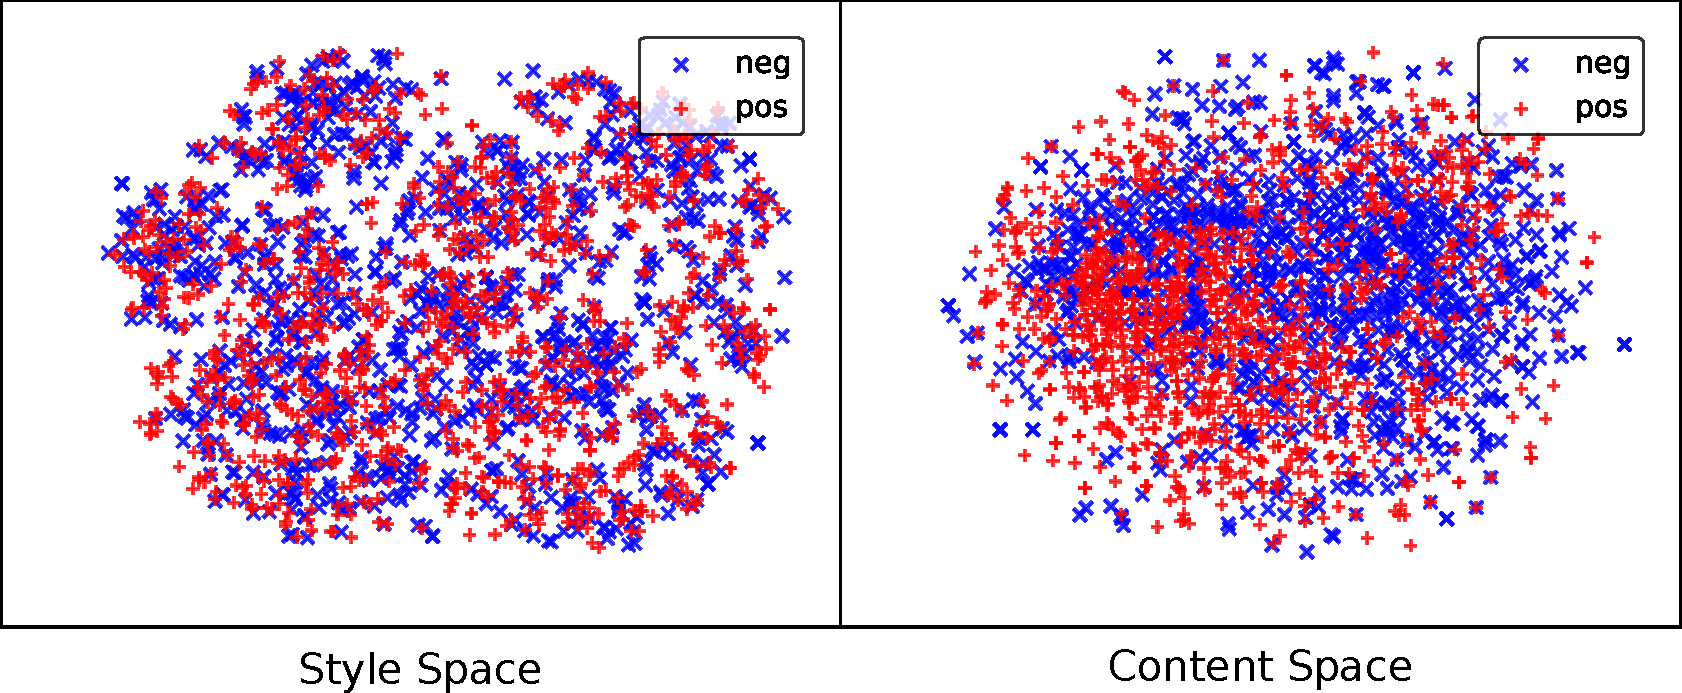
\includegraphics[width=\linewidth]{vae-latent-spaces-only-rec}
	\caption{t-SNE Plot of VAE latent embeddings with only $\loss{AE}$.}
	\label{fig:only-rec}
\end{figure}

\begin{figure}[ht]
	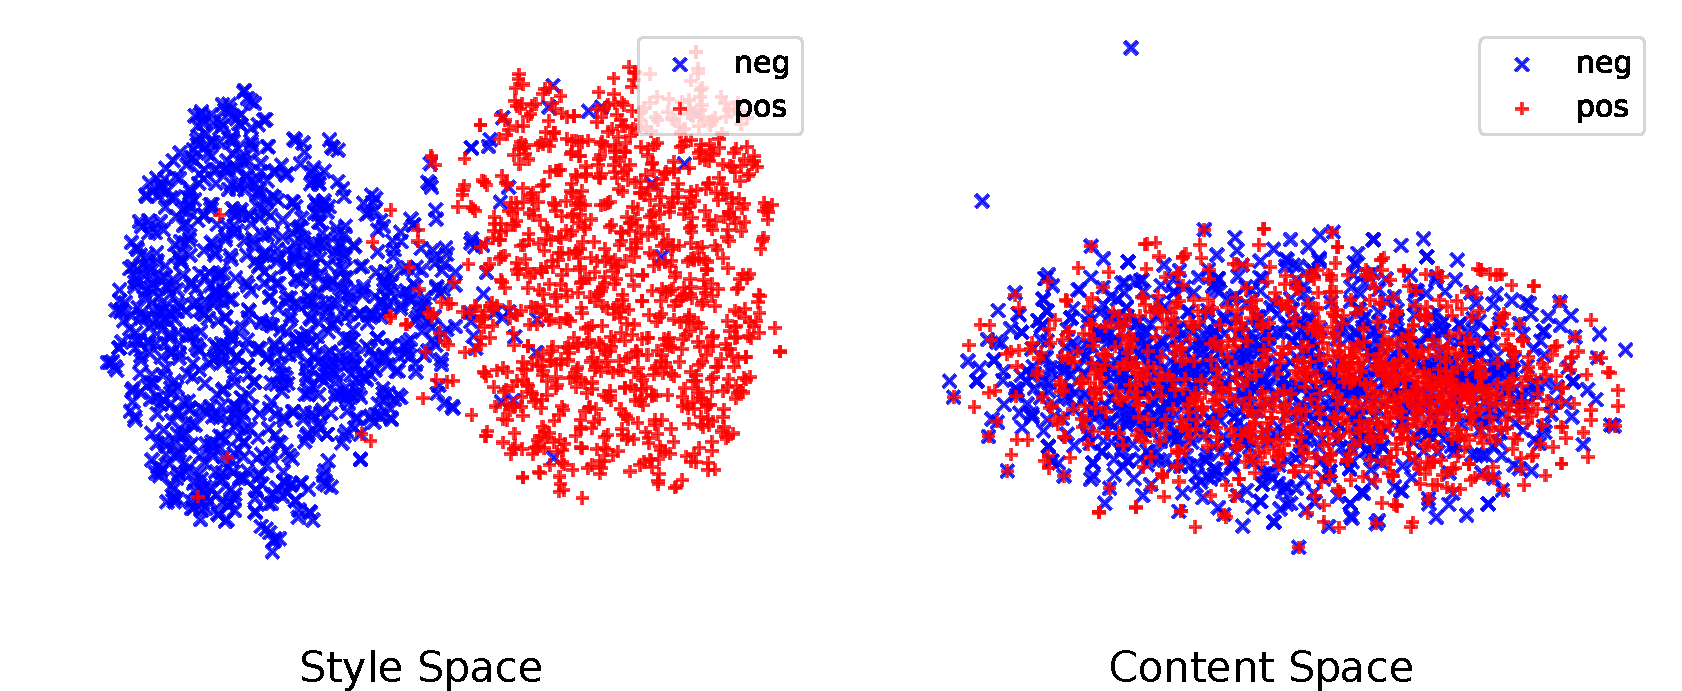
\includegraphics[width=\linewidth]{vae-latent-spaces-rec-muls}
	\caption{t-SNE Plot of VAE latent embeddings with $\loss{AE} + \loss{mul(s)}$.}
	\label{fig:rec-and-muls}
\end{figure}

\begin{figure}[ht]
	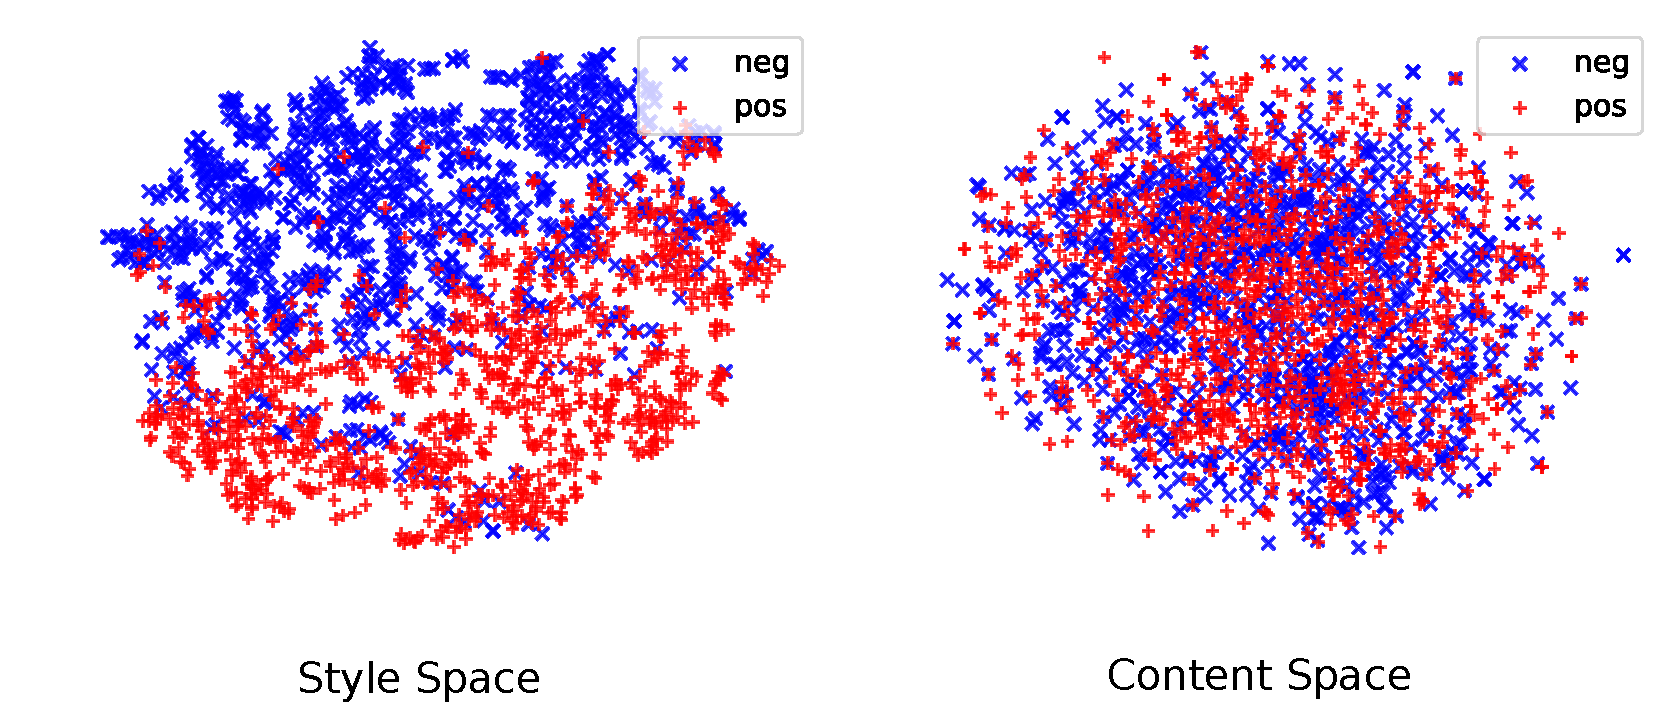
\includegraphics[width=\linewidth]{vae-latent-spaces-rec-advs}
	\caption{t-SNE Plot of VAE latent embeddings with $\loss{AE} + \loss{adv(s)}$.}
	\label{fig:rec-and-advs}
\end{figure}

\begin{figure}[ht]
	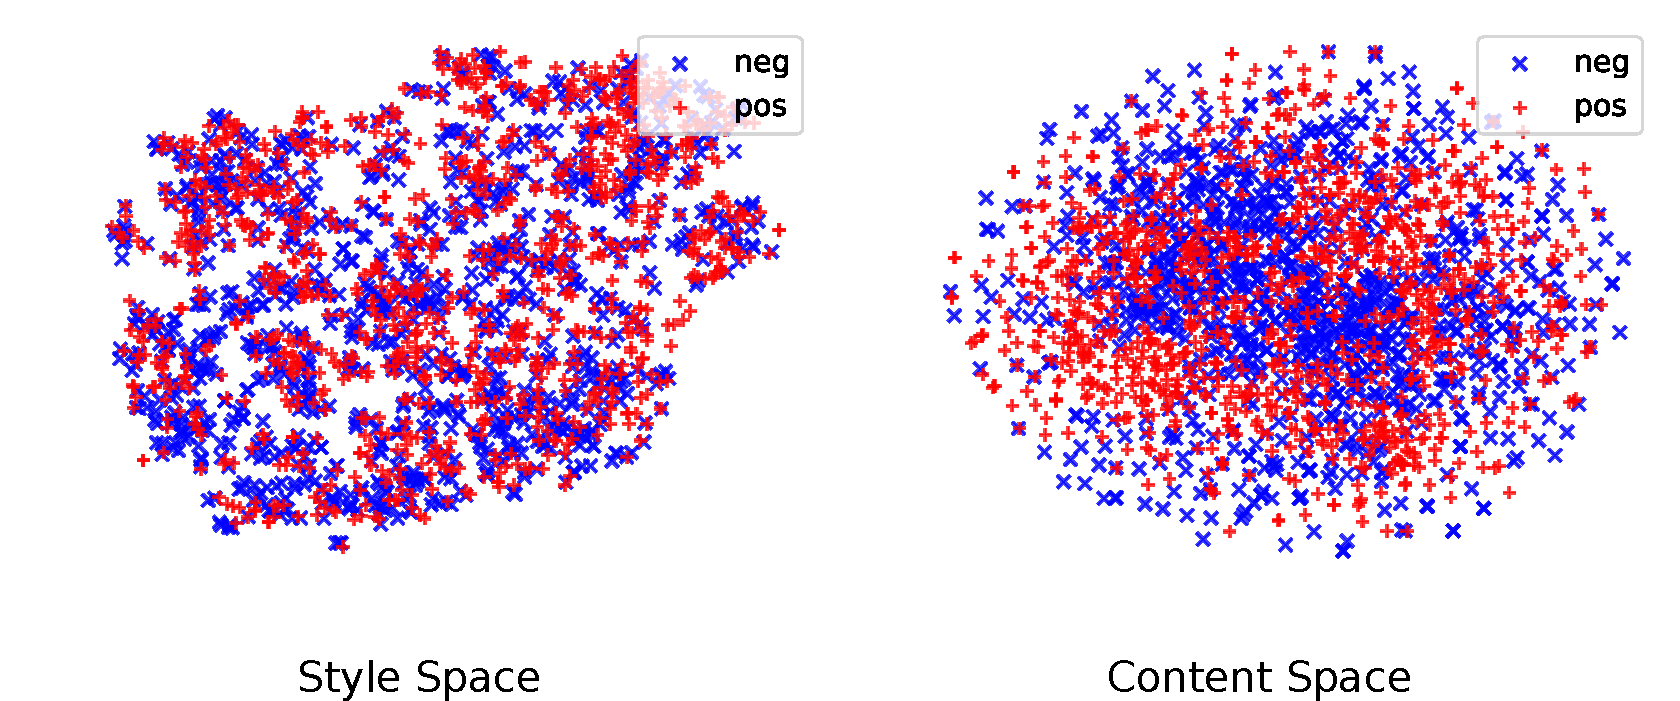
\includegraphics[width=\linewidth]{vae-latent-spaces-rec-mulc}
	\caption{t-SNE Plot of VAE latent embeddings with $\loss{AE} + \loss{mul(c)}$.}
	\label{fig:rec-and-mulc}
\end{figure}

\begin{figure}[ht]
	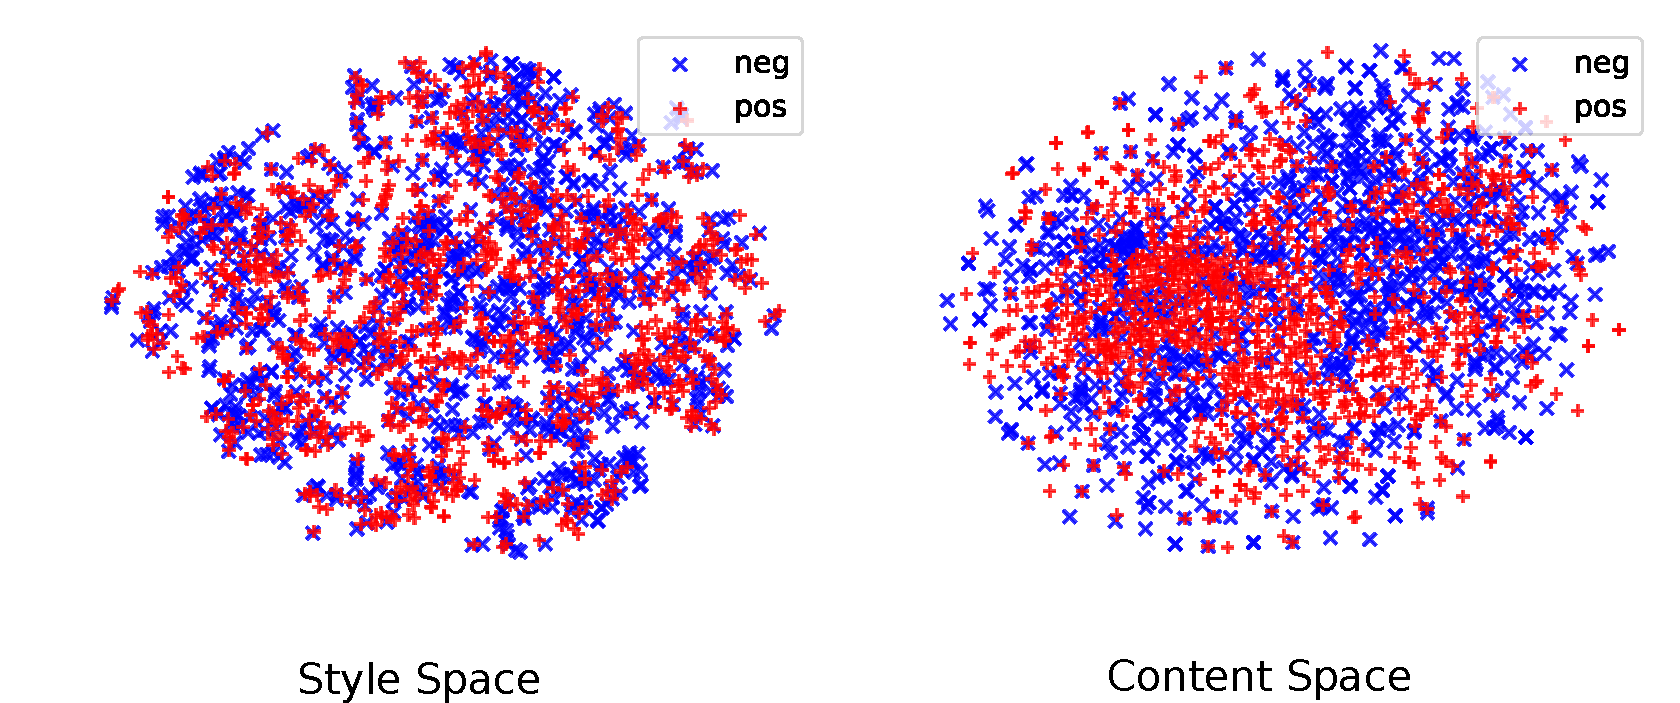
\includegraphics[width=\linewidth]{vae-latent-spaces-rec-advc}
	\caption{t-SNE Plot of VAE latent embeddings with $\loss{AE} + \loss{adv(c)}$.}
	\label{fig:rec-and-advc}
\end{figure}


\end{document}
